\documentclass[titlepage,a4paper]{article}

\usepackage{a4wide}
\usepackage[colorlinks=true,linkcolor=black,urlcolor=blue,bookmarksopen=true]{hyperref}
\usepackage{bookmark}
\usepackage{fancyhdr}
\usepackage[spanish]{babel}
\usepackage[utf8]{inputenc}
\usepackage[T1]{fontenc}
\usepackage{graphicx}
\usepackage{float}
\usepackage{hyperref}

\graphicspath{ {imagenes/} }  % Las imagenes las reubique en la carpeta imagenes

\pagestyle{fancy} % Encabezado y pie de página
\fancyhf{}
\fancyhead[L]{TP1}
\fancyhead[R]{Algoritmos y Programación III - FIUBA}
\renewcommand{\headrulewidth}{0.4pt}
\fancyfoot[C]{\thepage}
\renewcommand{\footrulewidth}{0.4pt}

\begin{document}
\begin{titlepage} % Carátula
	\hfill
\includegraphics[width=6cm]{logofiuba.jpg}
    \centering
    \vfill
    \Huge \textbf{Trabajo Práctico 1 — Smalltalk}
    \vskip2cm
    \Large [7507/9502] Algoritmos y Programación III\\
    Curso 2 \\ % Curso 1 para el de la tarde y 2 para el de la noche
    Primer cuatrimestre de 2020 
    \vfill
    \begin{tabular}{ | l | l | } % Datos del alumno
      \hline
      Alumno: & Paredes Ramirez, Luis José\\ \hline
      Número de padrón: & 104851 \\ \hline
      Email: & lparedesr@fi.uba.ar \\ \hline
  	\end{tabular}
    \vfill
    \vfill
\end{titlepage}

\tableofcontents % Índice general
\newpage

\section{Introducción}\label{sec:intro}
  El presente informe reune la documentacion del primer trabajo practico de la materia
  Algoritmos y Programación III que consiste en desarrollar un sistema que permita encontrar el mejor 
  presupuesto de un pintor de acuerdo a las necesidades de los clientes. \newline

  Este trabajo es desarrollado usando los conceptos del paradigma de la orientación a objetos
  utilizando el sistema Smalltalk.


% Deberá contener explicaciones de cada uno de los supuestos que el alumno haya tenido que adoptar a partir de 
% situaciones que no estén contempladas en la especificación.
\section{Supuestos}\label{sec:supuestos}

Los siguientes supuestos se tomaron como constantes que siempre se cumpliran en el trabajo practico.

  \subsection{Pincel}
    \begin{itemize}
      \item El pintor que utiliza Pincel siempre tarda 2 horas en pintar un $M^2$.
      \item El pintor que utiliza Pincel siempre gastara 4 litros por $M^2$.
      \item El pintor que utiliza Pincel dara un descuento del 50\% para proyectos mayores a 40 $M^2$.
    \end{itemize}

  \subsection{Rodillo}
    \begin{itemize}
      \item El pintor que utiliza Rodillo siempre tarda 1 horas en pintar un $M^2$.
      \item El pintor que utiliza Rodillo siempre gastara 5 litros por $M^2$.
      \item El pintor que utiliza Rodillo no aplica descuento para proyectos mayores a 40 $M^2$.
    \end{itemize}

  \subsection{Pintura}
    \begin{itemize}
      \item Si es negativo o cero: valor por $M^2$ o numero manos Pincel o numero manos Rodillo, entonces lanzara \textbf{ValorInvalido} al crear la pintura.
      \item Pintura Alba siempre requiere 1 mano con pincel o 1 mano con rodillo.
      \item Pintura Venier siempre requiere 2 manos con pincel o 1 mano con rodillo.
    \end{itemize}

  \subsection{Pintor}
    \begin{itemize}
      \item Se asume que siempre se cargaran pintores que no tengan nombres repetidos.
      \item Si el pintor pinta un numero negativo de $M^2$ se lanzara excepcion \textbf{ValorInvalido}.
    \end{itemize}
  

% Uno o varios diagramas de clases mostrando las relaciones estáticas entre las clases. 
% Puede agregarse todo el texto necesario para aclarar y explicar su diseño. 
%Recuerden que la idea de todo el documento es que quede documentado y entendible cómo está implementada la solución.
\newpage
\section{Diagramas de clase}\label{sec:diagramasdeclase}
%Uno o varios diagramas de clases mostrando las relaciones estáticas entre las clases.  
%Puede agregarse todo el texto necesario para aclarar y explicar su diseño. 
%Recuerden que la idea de todo el documento es que quede documentado y entendible cómo está implementada la solución. 
%Todos los diagramas tienen que estar embebidos como imágenes en el informe de manera tal que entren en el ancho de una hoja A4 
%sin tener que rotarla. No se aceptarán diagramas en archivos sueltos. 


% \footnote{Mensaje debajo}

\begin{figure}[H]
  \centering
  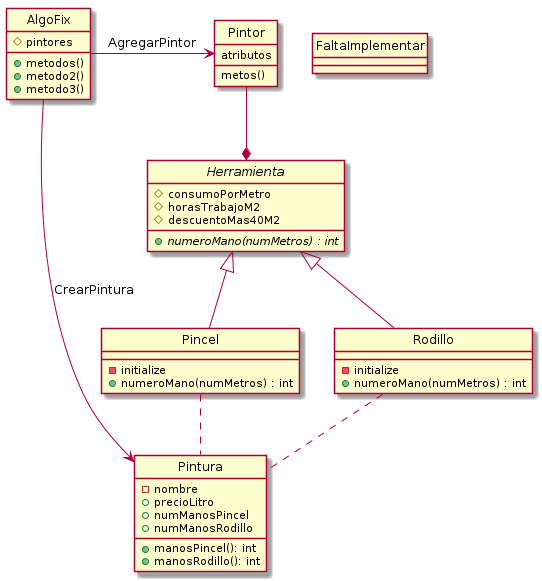
\includegraphics[width=0.8\textwidth]{diagrama_clase01.png}
  \caption{\label{fig:class01}Diagrama Asocioaciones entre Clases.}
  \end{figure}

  En el diagrama de la figura \ref{fig:class01} se observan las asociaciones entre las distintas clases. 
  Se observa que cada AlgoFix tendra por lo menos un pintor que siempre existirá junto con su herramienta, la cual puede ser Pincel o Rodillo. Esta tendrán el mismo
  comportamiento pero con sus propias propiedades. En particular, la herramienta definirá las horas que tendra que trabajar, junto con los Litros de pintura a gastar y 
  el descuento que hace (si es que hace) al pintar mas de 40 $M^2$ el Pintor. Cada pintor es responsable de conocer el precio que cobrará por el trabajo; por tanto, 
  al buscar el menor presupuesto se busca el pintor que cobre menos preguntandole a cada uno. 

\begin{figure}[H]
\centering
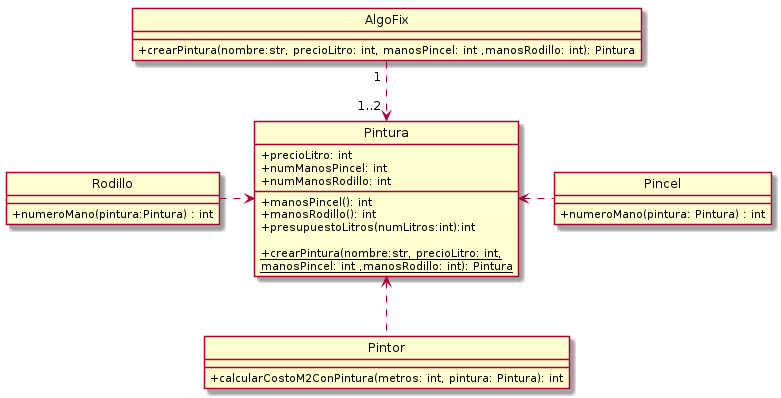
\includegraphics[width=1\textwidth]{diagrama_clase02.png}
\caption{\label{fig:class02}Diagrama de dependencias debiles con la clase Pintura.}
\end{figure}

En la figura \ref{fig:class02} se representan las dependencias debiles que tiene las distintas clases con la clase Pintura. Se separo del diagrama \ref{fig:class01} de modo que
 de aporte a una mayor claridad. Adicionalmente, como ya se incluyeron las distintas clases en el diagrama de la figura \ref{fig:class01} 
entonces se abstraen unicamente los metodos que hacen referencia al objeto Pintura.\newline

Dado que distintas pinturas requieren distintos trabajos, del diagrama se observa que el Pincel y Rodillo le preguntan cuantas manos deben pasar y el Pintor le pregunta
cuanto es el costo de la pintura segun los litros que se usó. Esto es debido a que la Pintura tiene comportamiento propio definido el cual solamente ésta conoce. 
Por ultimo, como a AlgoFix se le pide que cree una pintura entonces le delega el comportamiento al constructor de Pinturas y éste devuelve una con los datos establecidos.



% Explicaciones sobre la implementación interna de algunas clases que consideren que puedan llegar a resultar interesantes.
\section{Detalles de implementación}\label{sec:implementacion}
\begin{itemize}
  \item Por decisión de diseño las excepciones intentarán salir al no mas crear los objetos. Es decir, si en la creacion de un Pincel o Pintura se
  le pasa algun valor invalido lanzará la excepcion \textbf{ValorInvalido} en el momento de su creación. Sin embargo, adicionalmente para darle mayor 
  robustez al programa, en los casos bordes donde por alguna razon llega algun valor invalido a las operaciones esperadas, lanzara la 
  excepcion \textbf{ValorInvalido} y asi evitar resultados absurdos.
  
  \item Se tomaran los supuestos hechos en la sección \ref{sec:supuestos} como invariantes en todo momento del programa,
  por tanto las propiedades propias de cada objeto se asignan en su inicializacion en el momento de su creacion y no cambiaran.

  \item Al momento de refactorizar el codigo se observó que el comportamiento de \textbf{Pincel} y \textbf{Rodillo} es idéntico en todo excepto en el numeroManos. 
  Por tanto se tomo la decisión de crear una clase abstracta \textbf{Herramienta} que contenga el comportamiento en común y cada objeto define el numeroManos 
  necesario para pintar, según la pintura con la cual se trabaje.
\end{itemize}


\subsection{Nota de los tests}
De las pruebas integradoras, se extrajeron cada una de las pruebas unitarias y se pusieron en AlgoFixTestUnitarios 
de modo de simplificar el panorama y enfocar unicamente la atencion en resolver un problema a la vez. 
De este modo su proposito es cumplir con las pruebas por separado para que luego pasen las pruebas integradoras. \newline

Adicionalmente se creo una clase de prueba por cada clase creada para resolver el trabajo practico
en las cuales se pone a prueba el comportamiento esperado del objeto en tiempo de ejecucion. Por tanto
las pruebas de AlgoFix estan orientadas a que el objeto AlgoFix se comporte como es de esperar en tiempo de ejecucion, 
y es distinto de las otras pruebas.


% Explicación de cada una de las excepciones creadas y con qué fin fueron creadas.
\section{Excepciones}\label{sec:excepciones}
\begin{description}
\item[Exception \underline{ValorInvalido:}] Excepcion lanzada en caso de pasarle un parametro que no haga sentido para el comportamiento esperado del objeto
y evitar absurdos.

Se usa al pasarle un \textbf{numMetros} invalido al Pintor o a la Herramienta, y tambien cuando se pasa un \textbf{numLitros} invalido a la Pintura.
\end{description}


% Mostrar las secuencias interesantes que hayan implementado. Pueden agregar texto para explicar si algo no queda claro.
\section{Diagramas de secuencia}\label{sec:diagramasdesecuencia}

\subsection{test01ObtenerPresupuestoPintor}
En la figura \ref{fig:seq01} se muestra el diagrama de secuencia de los pasos para obtener el pintor de menor presupuesto.
El siguiente diagrama esta basado en el test01, sin embargo se devuelve el propio pintor ya que el actor no es SUnit y se 
trata de modelar un caso real donde el interés es calcular el pintor de menor presupuesto.

\begin{figure}[H]
\centering
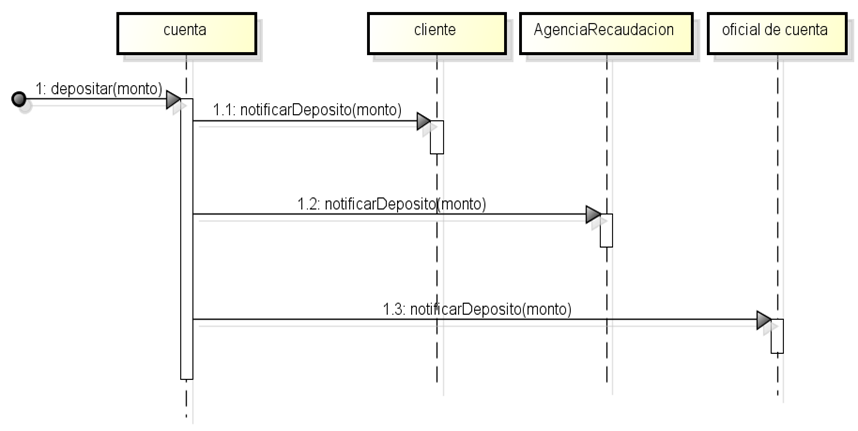
\includegraphics[width=0.98\textwidth]{diagrama_secuencia01.png} 
\caption{\label{fig:seq01}Comportamiento esperado para obtener pintor de menor presupuesto.}
\end{figure}

\newpage
\underline{Observaciones}
\begin{itemize}
  \item Se recortó el nombre del metodo \textbf{presupuestoMasBaratoParaPintarM2ConPintura}  a  \textbf{presupuesto...M2Pintura} para darle mayor claridad al diagrama.
  \item Cada pintor calcula el costo que tiene para hacer el trabajo. Se le pregunta cual es su valor y se va guardando el pintor de menor presupuesto para devolverlo.
  \item Los pasos que hace el pintor para calcular su presupuesto se abstrayeron en la figura \ref{fig:seq02} para darle claridad al diagrama.
\end{itemize}

\begin{figure}[H]
\centering
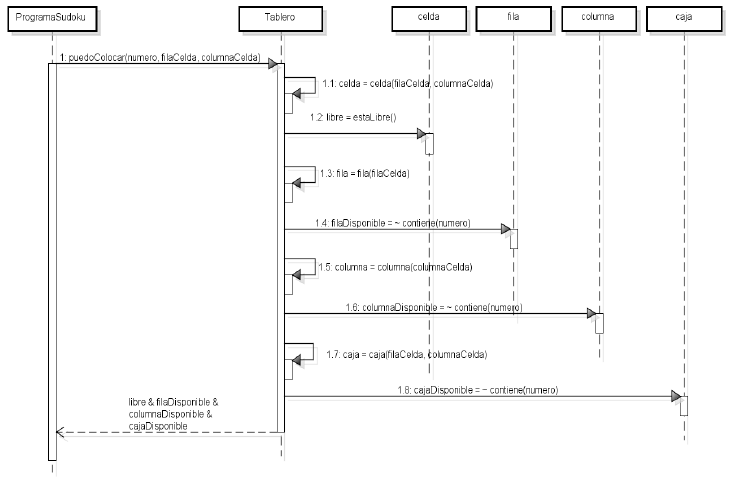
\includegraphics[width=\textwidth]{diagrama_secuencia02.png}
\caption{\label{fig:seq02} Diagrama de Secuencia de calcularCostoM2ConPintura(metros: int, pintura: Pintura).}
\end{figure}

\subsection{test04ObtenerDescuentoMas40M2}

Los siguientes diagramas modelan el test04 de las pruebas unitarias del pintor donde al pintar mas de
40 $M^2$ usando el Pincel y la pintura Alba entonces aplica un descuento del 50\%. En el diagrama \ref{fig:seq03} se 
grafica el caso feliz donde se cumplen las condiciones necesarias para aplicar el descuento y en el diagrama \ref{fig:seq04} 
se muestra que sucede en caso no cumplir las condiciones.

\begin{figure}[H]
  \centering
  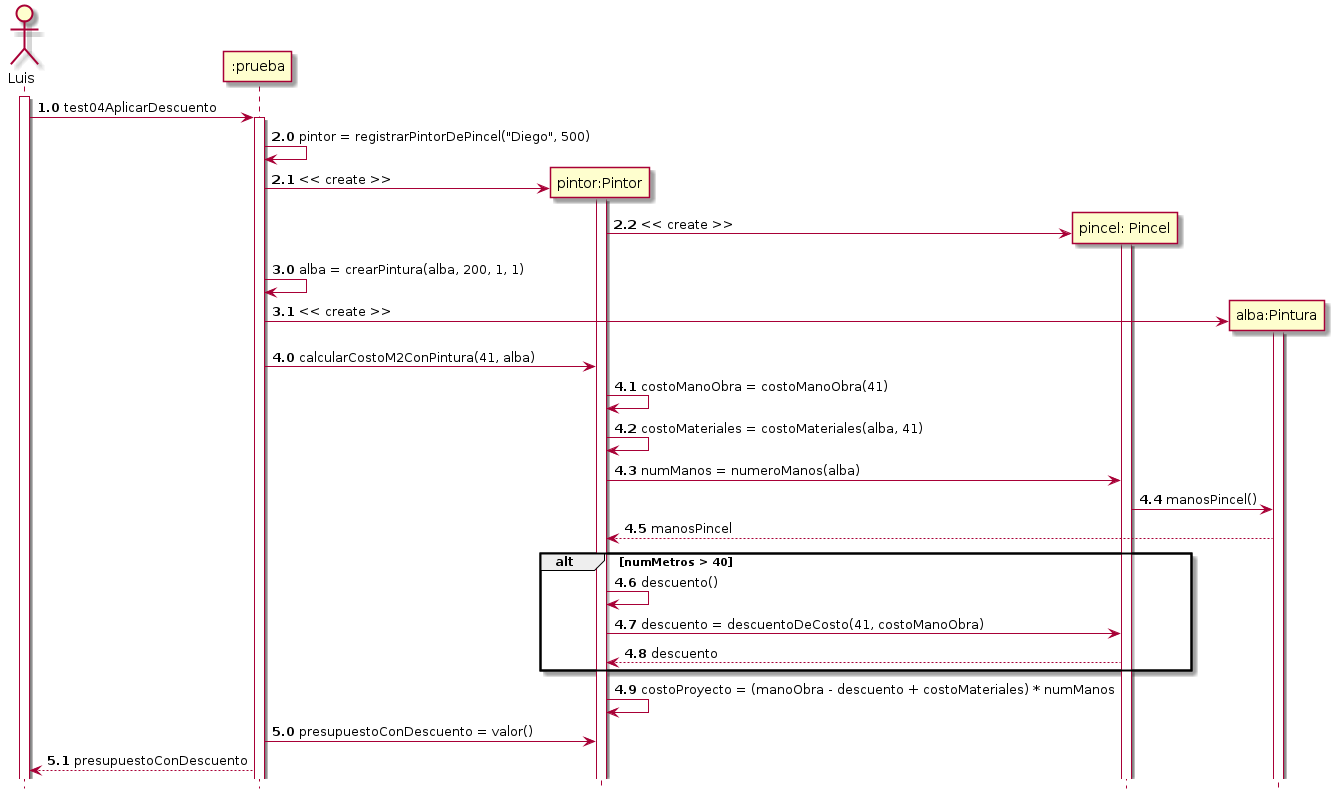
\includegraphics[width=0.9\textwidth]{diagrama_secuencia03.png}
  \caption{\label{fig:seq03}Diagrama de Secuencia del descuento. Caso Feliz.}
  \end{figure}

  De la figura \ref{fig:seq03} se destaca como principal característica que el pintor es quien decide si aplicar el descuento cuando se cumpla la condición necesaria. 
  En este caso se cumple y por tanto aplica el descuento; sin embargo, distintas herramientas aplicarán distintos 
  descuentos, entonces el pintor le pregunta a su herramienta (en este caso el Pincel) cuánto es el descuento que debe aplicar al monto original.

  Se omitieron las interacciones para los metodos costoManoObra(metros), costoMateriales(pintura,metros) ya que están 
  expresadas en la figura \ref{fig:seq02}

  \begin{figure}[H]
    \centering
    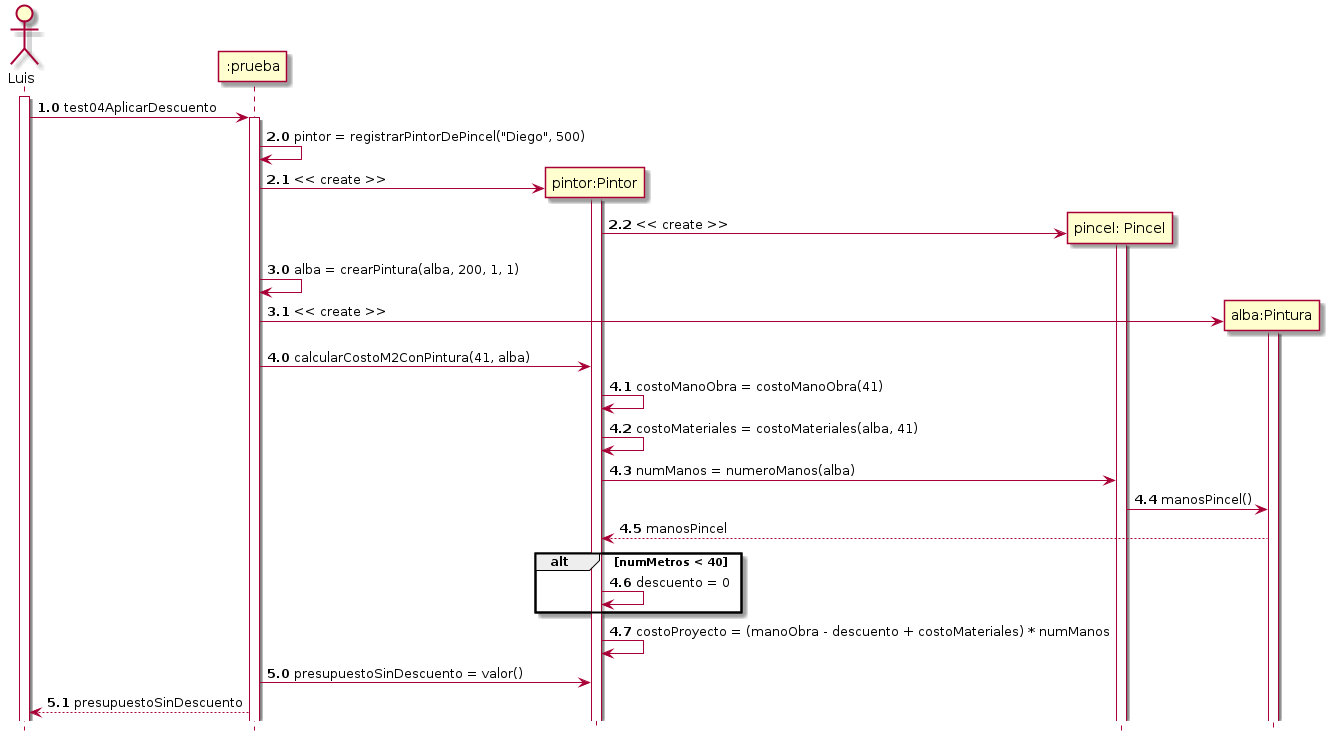
\includegraphics[width=0.9\textwidth]{diagrama_secuencia04.png}
    \caption{\label{fig:seq04}Diagrama de Secuencia donde no se aplica el descuento.}
    \end{figure}

    En la figura \ref{fig:seq04} el pintor no pinta mas de 40 $M^2$ entonces no aplica descuento.

\newpage
\section{Referencias}

\begin{itemize}
  \item UML gota a gota. Martin Fowler con Kendall Scott
  \item Texto de apoyo conceptual de Algoritmos y Programación III Facultad de Ingeniería de la Universidad de Buenos Aires. Carlos Fontela 2018
  \item Diagramas de Secuencia: \url{https://plantuml.com/sequence-diagram}
  \item Diagramas de Clase: \url{https://plantuml.com/class-diagram}
  \item Diagrama de Clase: \url{http://ogom.github.io/draw_uml/plantuml/}
  \item UML si o si: \url{https://campus.fi.uba.ar/mod/lesson/view.php?id=98901&pageid=2105&startlastseen=no}
  \item Documentacion para la herramienta LaTex: \url{https://www.overleaf.com/learn/latex/Main_Page}
\end{itemize}

\end{document}